
% Define listing style for yaml
\newcommand\YAMLcolonstyle{\color{black}\bfseries\small}
\newcommand\YAMLkeystyle{\color{black}\mdseries\small}
\newcommand\YAMLvaluestyle{\color{green}\mdseries\small}

\makeatletter

% here is a macro expanding to the name of the language
% (handy if you decide to change it further down the road)
\newcommand\language@yaml{yaml}

\expandafter\expandafter\expandafter\lstdefinelanguage
\expandafter{\language@yaml}
{
  keywords={true,false,null,y,n},
  keywordstyle=\color{darkgray}\bfseries,
  basicstyle=\YAMLkeystyle,                                 % assuming a key comes first
  sensitive=false,
  comment=[l]{\#},
  morecomment=[s]{/*}{*/},
  commentstyle=\color{purple}\ttfamily,
  stringstyle=\YAMLvaluestyle\ttfamily,
  moredelim=[l][\color{orange}]{\&},
  moredelim=[l][\color{magenta}]{*},
  moredelim=**[il][\YAMLcolonstyle{:}\YAMLvaluestyle]{:},   % switch to value style at :
  morestring=[b]',
  morestring=[b]",
  literate =    {---}{{\ProcessThreeDashes}}3
                {>}{{\textcolor{red}\textgreater}}1     
                {|}{{\textcolor{red}\textbar}}1 
                {\ -\ }{{\mdseries\ -\ }}3,
}

% switch to key style at EOL
\lst@AddToHook{EveryLine}{\ifx\lst@language\language@yaml\YAMLkeystyle\fi}
\makeatother

\newcommand\ProcessThreeDashes{\llap{\color{cyan}\mdseries-{-}-}}


\definecolor{codegreen}{rgb}{0,0.6,0}
\definecolor{codegray}{rgb}{0.5,0.5,0.5}
\definecolor{codepurple}{rgb}{0.58,0,0.82}
\definecolor{backcolour}{rgb}{0.95,0.95,0.92}

\lstdefinestyle{mystyle}{
    backgroundcolor=\color{backcolour},   
    commentstyle=\color{codegreen},
    keywordstyle=\color{magenta},
    numberstyle=\tiny\color{codegray},
    stringstyle=\color{codepurple},
    basicstyle=\ttfamily\footnotesize,
    breakatwhitespace=false,         
    breaklines=true,                 
    captionpos=b,                    
    keepspaces=true,                 
    numbers=left,                    
    numbersep=5pt,                  
    showspaces=false,                
    showstringspaces=false,
    showtabs=false,                  
    tabsize=2,
    xleftmargin=15pt
}

\lstset{style=mystyle}

\chapter{Implementation} \label{chp:Implementation}
To evaluate how reinforcement learning performs when being faced with the problem of distributed particle navigation we needed to implement a number of components: A simulation for the particles and mazes to test which allows feedback to the RL algorithm, an experimentation environment, which lets us test RL algorithms with different parameters on the simulation and an evaluation component, which monitors the performance during and after training.

In this chapter, we will begin by presenting our flexible experimentation framework called \textit{Baselines-Lab} in Section \ref{sec:BaselinesLab}. This framework implements an easy-to-use laboratory environment for RL experiments, which is completely controllable by configuration files and command-line arguments and allows the user to customize RL algorithms for \textit{any} problem. The framework uses the reinforcement learning library \textit{stable-baselines} \cite{stable-baselines} as backend infrastructure and thus offers many high-quality implementations of RL algorithms for testing. Baselines-Lab also extends stable-baselines with components like curiosity, automated hyperparametersearch, or a flexible neural network generation system. All in all, Baselines-Lab is designed to offer an easy way to train, monitor and evaluate deep RL agents under a given problem. We will later use Baselines-Lab for all our experiments in Chapter \ref{chp:Evaluation}. 

To perform experiments on the particle navigation problem, we need an implementation which simulates the maze and the particles. This simulation needs to be as fast as possible, because RL algorithms will need to simulate millions of steps during training. We also needed an environment which is customizable in every aspect, to allow us to experiment with different reward settings, randomized mazes, randomized goal positions or different particle behavior. We implemented this particle simulator along with a modular system for environment customization and provide implementation details in in Section \ref{sec:MazeEnvironment}. 

\section{General Implementation Notes} \label{sec:ImplementationNotes}
Before dive into the actual implementation we want to talk a little bit about our general design choices. As a programming language we chose to use Python 3 \cite{van2011python, pythonWebsite}. Python is an interpreted high-level programming language. Even though it is interpreted and thus may be slower than a direct implementation in C or C++, the easy integration of high-performance libraries which also scale into distributed systems make applications developed in python very fast. In the past years many ML library have been developed for python making Python an ideal choice for data-science and machine learning projects.

To date, we have the choice between several machine learning libraries which all support the creation and training of artificial neural networks. Modern libraries also especially leverage the computing power of the GPU to accelerate computation. Many of the libraries support more or less the same functionality, but may have a very different style of how certain things can be achieved. Currently the two most popular libraries for machine learning (with Python) are PyTorch \cite{paszke2019pytorch} and Tensorflow \cite{abadi2016tensorflow}. For this project we decided to use Tensorflow in version 1.14. This decision was made in conjunction with our second big backend library which extends Tensorflow for reinforcement learning: Stable-Baselines \cite{stable-baselines}. Stable baselines offers high-quality implementations of many RL algorithms which are partially forked from the OpenAI Baselines project \cite{baselines}. While Google offers their own reinforcement library as a Tensorflow extension named TF-Agents \cite{TFAgents} we found that it currently is in a too early development state and thus not stable enough.

Since Python offers the easy integration of additional libraries we also make use of a number of additional libraries, most notably:
\begin{itemize}
    \item OpenAI Gym \cite{openAIgym} for a standardized environment creation as well as the integration of the Atari environments for testing purposes.
    \item OpenCV \cite{opencv_library} for image preprocessing.
    \item NumPy \cite{oliphant2006guide} for fast matrix computations.
    \item Optuna \cite{akiba2019optuna} for automated hyperparameter search.
\end{itemize}

We provide a complete list of all libraries and their respective version which were used in this project in Appendix \ref{apx:BaselinesLab}.  

\section{Baselines Lab} \label{sec:BaselinesLab}
To test various combinations of reinforcement learning algorithms, their settings with different environments and environment settings, we need a flexible and easy configurable program which also gives us the possibility to monitor the performance and create evaluations of trained models. 

While there already exist some projects which offer some of these features, we did not find a project which was fully suited for our needs. The stable-baselines co-project baselines zoo \cite{rl-zoo} had to few options for the configuration of algorithms and while other libraries like slm-lab \cite{kenggraesser2017slmlab} did fit our needs for configurability, they did not offer enough integrated reinforcement learning algorithms. Therefore we decided to build our own lab environment on top of stable-baselines which we therefore call \textit{Baselines Lab}.

\subsection{Basic Features} \label{sec:blFunctions}
In this section, we want to go over the basic features of Baselines Lab. When starting the lab, we have to choose between one of the three different lab modes:

\begin{enumerate}
    \item The \textit{train} lab mode can be used to train a new model.
    \item The \textit{enjoy} lab mode can be used to watch a model in action and/or evaluate its performance.
    \item The \textit{search} lab mode can be used to perform an automated hyperparametersearch. We will talk more about the search mode in Section \ref{sec:blSearch}.
\end{enumerate}

When starting a session, we also need to specify a \textit{lab configuration file} which can be written in JSON or YAML. Let us take a look at the easiest form of a config file which specifies all mandatory parameters:

\begin{figure}[h]
    \lstinputlisting[language=yaml]{figures/implementation/simple_config.yml}
    \caption[Basic lab configuration file]{Basic lab configuration file in YAML.}
    \label{fig:BasicLabConfig}
\end{figure}


We can see that the basic lab configuration only requires a handful of parameters which define which RL algorithm should be used in conjunction with which neural network and which environment. Additionally we have to specify how long the agent should be trained. 

In general there are three basic categories for the parameters defined by the three main keywords: 

\begin{enumerate}
    \item The \textit{algorithm} keyword specifies all parameters related to the reinforcement learning algorithm. The parameters which can be set are algorithm dependent and directly correspond to the parameters of the stable-baselines documentation \cite{stable-baselines-docs}. The only exception to this is the \textit{policy} keyword, which defines the used neural network. We can use any registered policy type by using the \textit{name} keyword. Additional policy arguments can be directly specified as children of the \textit{policy} keyword.
    \item The \textit{env} keyword specifies all parameters which are directly related to the environment. The only mandatory parameter is the name of the environment corresponding to its registered gym entry. The env keyword allows for a lot of parameters regarding observation preprocessing like frame stacking or normalization. We included a full list in Appendix \ref{apx:BaselinesLab}. 
    \item  The \textit{meta} keyword describes all additional parameters related to the training process. For example we can define how often the model should be saved or evaluated, which random seed should be used or how many times the experiment should be repeated. For a full list of available arguments, see Appendix \ref{apx:BaselinesLab}.
\end{enumerate}

The same configuration file can be used for all lab modes. However some keywords may only take effect in a certain lab mode. By specifying a log directory, we can monitor the training process and periodically save the model during training. The latest or best models can then be inspected in enjoy mode by starting the lab with the same configuration file. 

\paragraph{Automated Saving and Loading.}
Given a log directory, Baselines Lab will automatically save models during training. Saving a model is complicated, since the model may need more than the network parameters to be correctly loaded in the future - either for inspection or extended training. For example if we normalized the observations of the environment using a running mean, we need to save that running mean, otherwise our model would not be able to perform later on. A single checkpoint therefore may contain multiple files depending on the current configuration.

If a log directory location is specified the lab will create a log directory with a current timestamp. Models (and additional components) will be periodically saved during training to a subdirectory called \textit{checkpoints}. On default, the lab keeps the last 5 checkpoints \textit{and} the model which had the best performance during training. This behavior can also be changed (see Appendix \ref{apx:BaselinesLab}).

The checkpoints created during training can be used in enjoy mode or if we want to continue training in the future. To continue training, we just add a \texttt{trained\_agent} keyword to the algorithm configuration and specify weather we want to load the \textit{last} or the \textit{best} checkpoint. In enjoy mode the best checkpoint is selected on default. To change this behavior we can specify a \texttt{-{}-type} command line argument and set it to \textit{last}.

\paragraph{Automated Evaluation}
Models are automatically evaluated during training. This evaluation is done periodically to determine the current model performance. Evaluation can be done in three different modes depending on the desired tradeoff between evaluation accuracy and speed:

\begin{enumerate}
    \item \textbf{Fast.} In fast evaluation mode, the lab is not performing a dedicated evaluation run. Instead the current results are computed by looking at the average reward and episode length over the last 100 training episodes. This procedure is very fast because the results are already computed during training, but may be inaccurate and also include the training behavior of the agent, which might be substantially different from its test behavior depending on the used RL algorithm (e.g. for DQN).
    \item \textbf{Normal.} In normal evaluation mode, the lab uses a dedicated vectorized evaluation environment with 32 parallel instances. Because each instance is reset independently this evaluation type still might produce a small bias towards short episodes, which slightly improves results if short episodes are good and slightly worsens results if short episodes are bad. Nevertheless we found that the results do not deviate too much from the results when executing the same model on a single environment and thus the results can be used to compare different models.
    \item \textbf{Slow.} In slow evaluation mode, the lab uses a dedicated evaluation environment with a single instance. This might take a lot of time during training, but produces the most accurate evaluation results. 
\end{enumerate}

Evaluation during training is used to determine the current best model and for monitoring purposes. To evaluate models outside of the train lab mode, we can use the enjoy lab mode. By specifying the \texttt{-{}-evaluate} command line argument, the lab creates a file at the log directory location containing detailed evaluation results. The argument expects a number of episodes and uses the normal evaluation mode on default. If we are interested in completely accurate results, we can additionally specify the \texttt{-{}-strict} option. 

\paragraph{Monitoring}
Monitoring the training process is very important for machine learning. By logging all kinds of values, we are able to determine errors in the implementation, select good hyperparameters and overall control the quality of the training process. Luckily, Tensorflow comes with an integrated monitoring system called Tensorboard which allows us to inspect the neural network and log values during training. These values can then be plotted in real time by starting the Tensorboard web server application. Figure \ref{fig:TensorboardExample} shows an example of the Tensorboard visualization, which can be accessed with a web browser.

\begin{figure}[ht]
    
    \begin{center}
        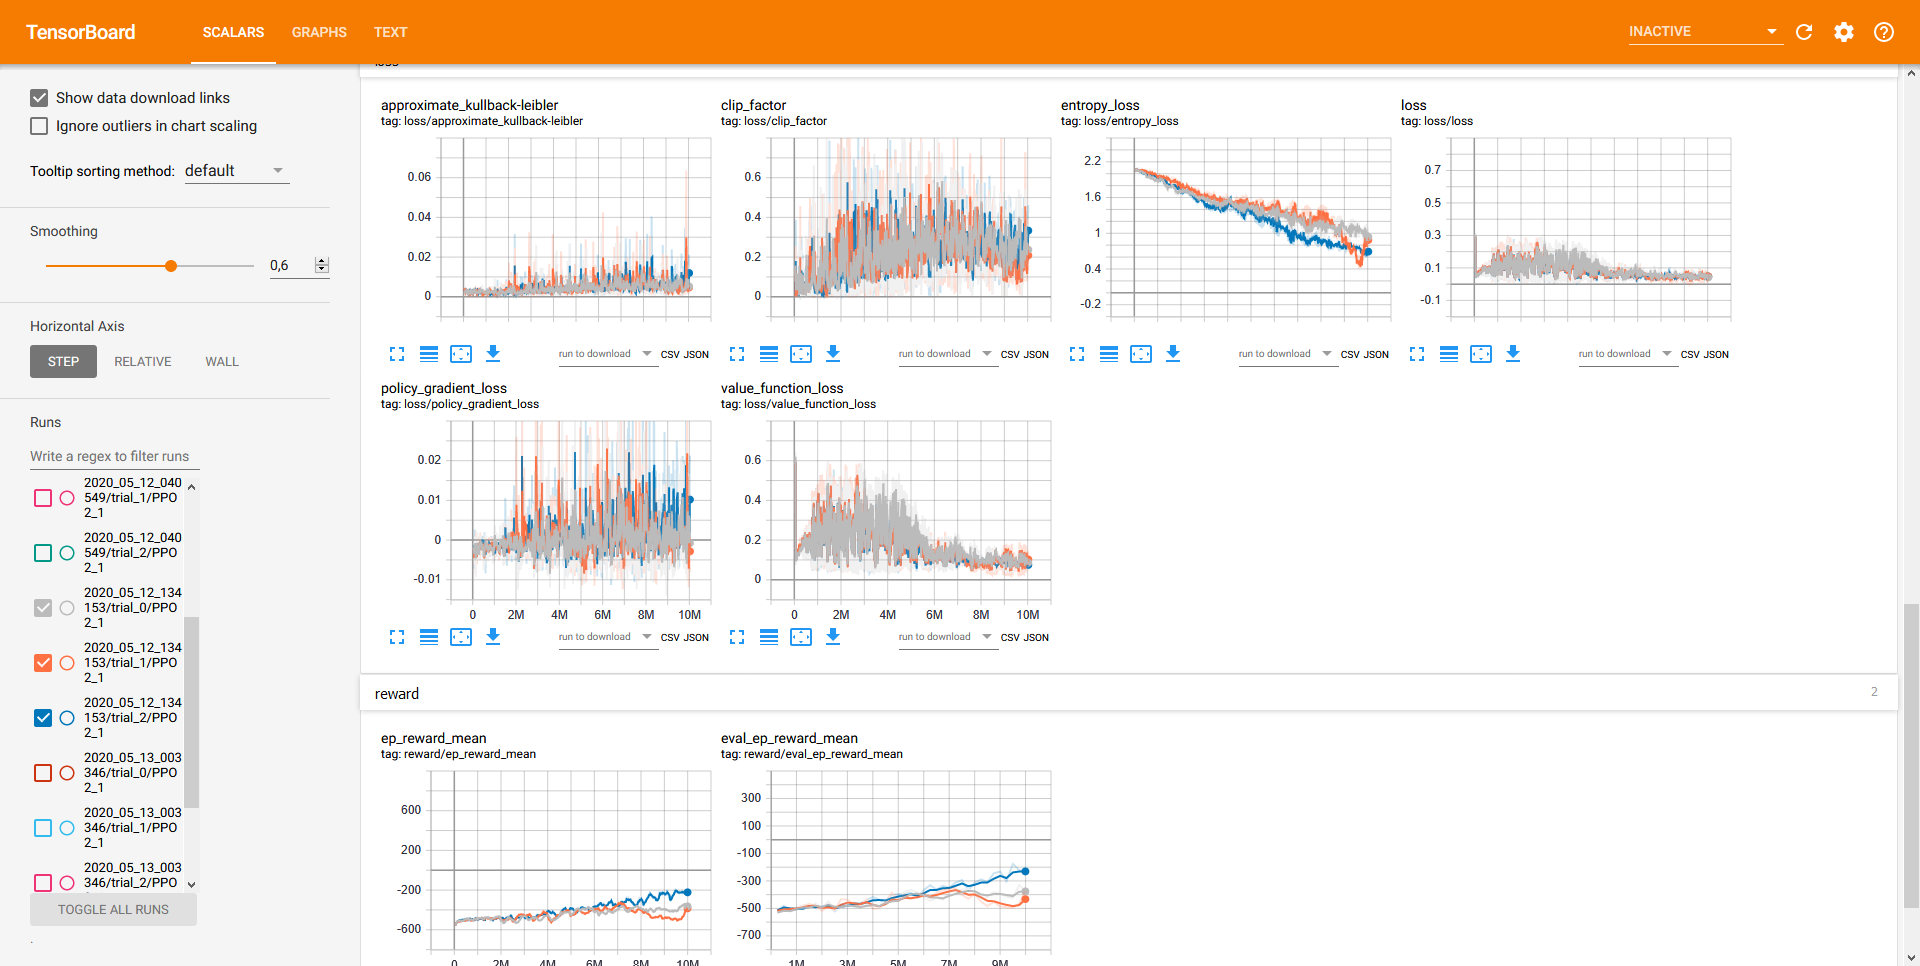
\includegraphics[clip, width=0.95\columnwidth]{figures/implementation/Tensorboard.png}
    \end{center}
    
    %\vspace*{-6pt}
    \caption[Tensorboard Example]{Example for a Tensorboard visualization.}
    \label{fig:TensorboardExample}
    %\vspace*{-12pt}
  \end{figure}

Stable Baselines already integrates Tensorboard for extended logging and visualization. Dependent on the chosen RL algorithm, Stable Baselines will log internal values like the average action advantage or the discounted reward. With Baselines Lab, we extend these logging capabilities and now also include several new values:

\begin{itemize}
    \item Smoothed episode length and episode reward for both training and evaluation.
    \item Special values - e.g. intrinsic and extrinsic reward when using the RND wrapper.
    \item The lab configuration as text. This is handy in situations, where Tensorboard visualizes multiple runs at once.
    \item Periodic images showing the state of the environment or the observations. This makes it easy to see what strategies the agent has learned without executing the agent in train lab mode.
    \item Frames per second to monitor training performance.
\end{itemize}

Tensorboard logs are created automatically at the given log directory location if the \texttt{tensorboard\_log} parameter of the algorithm is set to true. Some values like periodic images require additional opt-in since they may require a lot of disc space. See Appendix \ref{apx:BaselinesLab} for more information.

\paragraph{Extension of Stable Baselines Functions.}
Additional to the extended monitoring, we also extended some other functions of Stable Baselines:

\begin{itemize}
    \item \textit{Learning Rate Schedules.} Stable Baselines includes an inconsistent system of learning rate schedules, which are only available for certain algorithms. In Baselines Lab we therefore included linear and piecewise learning rate schedules for the PPO, SAC and TD3 implementations. For information on how these schedules can be used we included an example in Appendix \ref{apx:BaselinesLab}.
    \item \textit{Flexible Neural Network Creation.} Stable Baselines only allows to flexibly create dense neural networks. We extended the network base classes to also include a fully configurable network class which can be defined via config files. For an example see Appendix \ref{apx:BaselinesLab}.
\end{itemize}


\subsection{Random Network Distillation Module} \label{sec:blRND}
Stable Baselines does not offer an implementation for any form of curiosity reward. Since Huang et al. had shown, that curiosity reward can significantly improve training, we needed to implement our own version of intrinsic reward. In all previous experiments the RND curiosity reward produced superior results in comparison with the original idea of an ICM module. We therefore decided to implement the RND reward. 

\begin{figure}[ht]
    \begin{center}
    %\resizebox{0.95\columnwidth}{!}{%
    \begin{tabular}{c}
    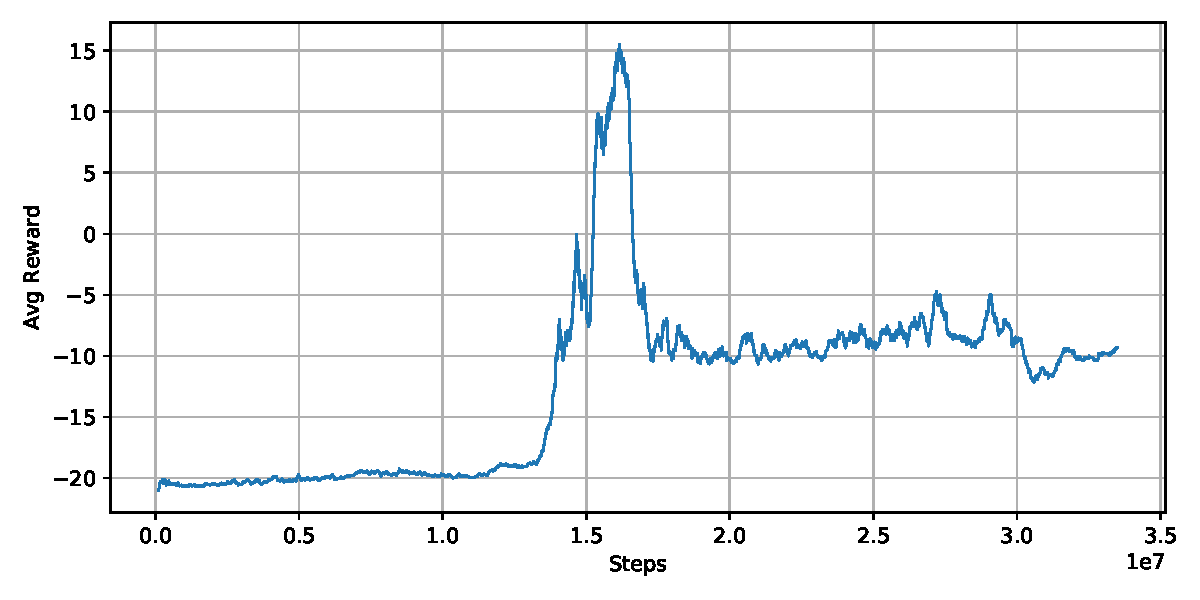
\includegraphics[clip, height=4.5cm]{figures/implementation/rnd_pong_episode_reward.pdf} \\
    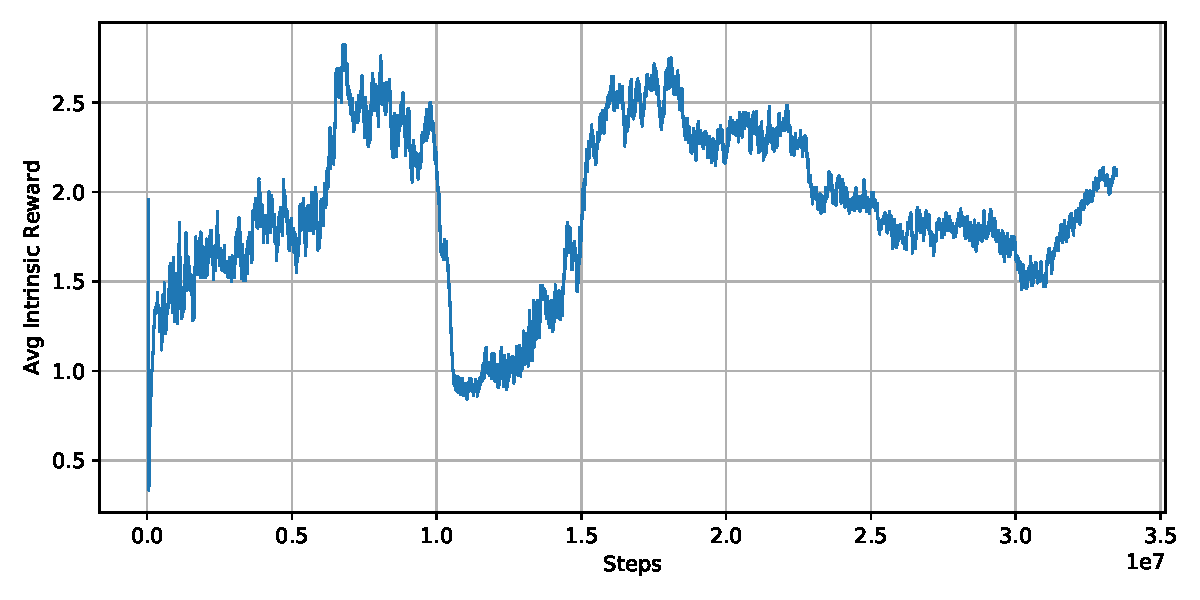
\includegraphics[clip, height=4.5cm]{figures/implementation/rnd_pong_episode_intrinsic_reward.pdf} \\
    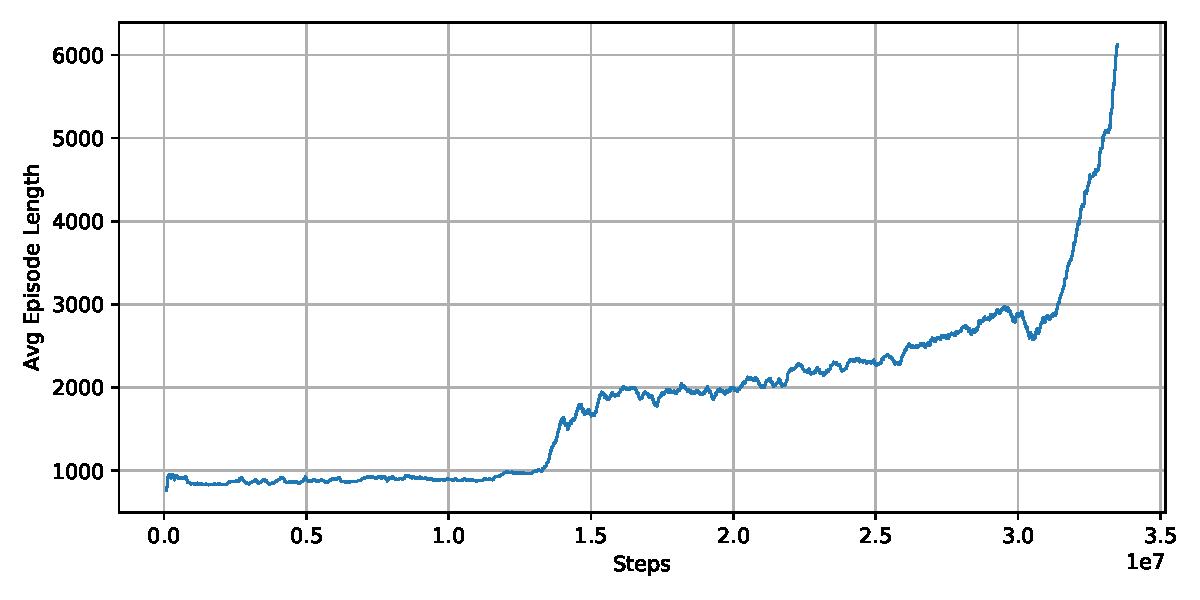
\includegraphics[clip, height=4.5cm]{figures/implementation/rnd_pong_episode_length.pdf} \\
    
    \end{tabular}
    %}%
    \end{center}
    %\vspace*{-12pt}
    \caption[RND on Pong]{Learning curves for the verification experiment of the curiosity reward wrapper on the Atari game Pong.}
    \label{fig:RNDPong}
    %\vspace*{-12pt}
  \end{figure}


Instead of implementing the curiosity reward as an extension of PPO (like in the original implementation) we decided to implement RND as a wrapper for the environment. This wrapper contains an internal replay buffer which contains samples from the past four training periods. On default, we train the predictor network with the same frequency as the actor network. For example, if we train 256 steps on 16 environments between each training period of the actor, the replay buffer will have a size of $256 \times 16 \times 4 = 16384$ samples. When training the predictor, we randomly draw batches of $0.25*\text{size(buffer)}$ from the buffer. On default, we perform four optimization epochs. The networks used for the target and predictor network have the same structure as in the original implementation.

The implementation of the RND module as a wrapper allows us to use the curiosity reward signal independent of the RL algorithm. We verified our implementation by training an PPO agent to play the Atari game "Pong" using curiosity reward only and no end-of-episode signal. Figure \ref{fig:RNDPong} shows the learning curves for intrinsic and extrinsic reward, as well as the episode length. We can see, that the agent does not optimize for extrinsic reward - this is expected, since we removed that reward signal - and instead continuously improves the intrinsic reward by increasing the episode length. The agent therefore learns to play with its enemy in Pong instead of against him. This behavior was also observed by Burda et al.\cite{burda2018exploration}.

The development of the curiosity wrapper was done in collaboration with the development team of Stable Baselines, and the implementation has been staged for a future release of Stable Baselines 3 \cite{stable-baselines-intrinsic}.

\subsection{Automated Hyperparametersearch} \label{sec:blSearch}
The choice of optimal hyperparameters is very important in any machine learning setting. As we saw in Chapter \ref{chp: RLOverview}, most RL algorithms introduce multiple new parameters, with some of them having great influence on the training performance. These parameter must be tuned additional to the already existing hyperparameters like the learning rate or other optimizer specific values, an observation preprocessing pipeline and eventual environment parameters (e.g. for reward generation). Tuning all these parameters together is especially hard, because every training run may take hours before we can determine if the current configuration is better or worse than any other configuration. To support our decisions when tuning these parameters, we therefore need the possibility of an automated hyperparametersearch. 

\begin{figure}[ht]
    \lstinputlisting[language=yaml]{figures/implementation/simple_search_config.yml}
    \caption{Basic search lab configuration file.}
    \label{fig:BasicSearchConfig}
\end{figure}

To efficiently search for hyperparameters in an ML context, a number of algorithms have been developed in the past which all have their individual strengths and weaknesses. Modern optimizer frameworks therefore often allow to choose between a number of different algorithms. For Baselines Lab, we choose to integrate Optuna \cite{akiba2019optuna} as it combines a number of up-to-date algorithms with great configurability. In Optuna there are mainly two classes of important algorithms: Samplers and Pruners. Samplers are used to choose from a set of hyperparameters and pruners are used to decide which trial should be canceled early (pruned). While both classes can be used with simple algorithms (e.g. a random value sampler with a median pruner), in Optuna we also can choose from more advanced algorithms. For example sampling can be done using the tree-structured parzen estimator algorithm \cite{bergstra2011algorithms} or pruning can be done via successive halving \cite{karnin2013almost}.

With Baselines Lab we can now configure the hyperparametersearch via config files. In Figure \ref{fig:BasicSearchConfig} we included an example showing an excerpt of a lab configuration. The shown section for the \textit{search} keyword can be appended to the lab configuration from Figure \ref{fig:BasicLabConfig} and is only used if the file is started with the \texttt{search} lab mode. We can see that we can define how many different configurations should be tested via the \texttt{n\_trials} keyword and that we can define a sampler and a pruner method. Each pruner can receive its individual parameters by specifying them as children of the \texttt{pruner} keyword. For example the \textit{halving} pruner gets configured such that each trial will run for at least 4000 timesteps before it can be pruned.

Depending on the chosen RL algorithm, Baselines Lab comes with a predefined set of parameter ranges which will automatically be sampled. Parameters which are explicitly given via the normal algorithm or env keyword will not be changed during the parametersearch. If we want to include additional parameters, we can define them under search/algorithm or search/env with a sampler method and the according choices. More details can be found in the Optuna documentation \cite{optuna-docs} and in Appendix \ref{apx:BaselinesLab}.

\subsection{Additional Features} \label{sec:blAdvanced}
Baselines Lab offers a bunch of additional functions which are designed to help monitoring the training process, find problems with the learning algorithm and help with result presentation:

\begin{itemize}
    \item \textit{Plots.} Baselines Lab can automatically create plots of the tensorboard training data. To create the plots either specify \texttt{plot: true} under the \texttt{meta} keyword or use the \texttt{-{}-plot} command line argument in enjoy mode. The default plots contain train and evaluation data for reward and episode length, but it is possible to plot additional data by specifying their tensorboard tags. For more information see Appendix \ref{apx:BaselinesLab}.
    \item \textit{Video Creation.} Baselines Lab can automatically create videos of  the environment. The environment can either be rendered like it is displayed in enjoy mode or the environment can render the observations which are created for the agent. Both options are only available in enjoy mode and can be enabled with the command line arguments \texttt{-{}-video} or \texttt{-{}-obs-video} respectively.
    \item \textit{Email Notification.} Baselines Lab can automatically send email notifications to send updates about the training progress. This feature is only available on Linux and requires \textit{mailx} to be installed. To send email notifications we have to specify a mail address via the \texttt{-{}-mail} command line argument. 
\end{itemize}


\subsection{Example Usage} \label{sec:BLExampleUsage}
In this section, we want to give a complete example, of how Baselines Lab can be used to train an RL agent on a novel environment. 

\paragraph{Creating the Environment.} Before training an agent, we must implement an environment which handles the interaction with the agent. To allow creators of RL algorithms and creators of RL problems to have a unified interface, OpenAI released a standardized format, together with a collection of some of the most used RL problems called \textit{OpenAI Gym} \cite{openAIgym}. Baselines Lab requires environments to implement this standard. Every environment must inherit from \texttt{gym.Env} and define the following four methods:

\begin{itemize}
    \item \texttt{step(action)} which allows the agent to interact with the environment by specifying an \textit{action} and receiving a tuple of (observation, reward, done, info) in return. Done indicates if the episode is over and info may contain additional information. If the environment is done it needs to be reset manually by calling \texttt{reset}.
    \item \texttt{reset()} which resets the environment to a initial state (which is usually randomized) and returns the initial observation.
    \item \texttt{render()} which allows us to render the environment in form of an rgb image intended for the user to display.
    \item \texttt{seed(seed)} which allows to set a random seed to generate reproducible results. 
\end{itemize}

Environments are usually registered within the gym registry and can then be created by specifying their unique name or id to \texttt{gym.make()}. The interface allows to provide extra arguments to the environment on creation to allow environment customization. For more information on environment creation or how to use environment methods, please refer to the Gym documentation at \cite{openAIdocumentation}.

\begin{figure}[p]
    \begin{center}
        \inputpython{figures/implementation/code/number_env.py}{0}{39}
    \end{center}
    \caption[Example Implementation of a Simple Environment]{Example environment implementation using the OpenAI gym interface. The goal for the agent is to increment or decrement a random number until it matches a second random number as fast as possible, by choosing from the actions (+1, +5, +10, -1, -5, -10). Note that we omitted an implementation for the \texttt{render} method, which should display the environment visually.} \label{fig:EnvironmentExampleImplementation}
\end{figure}

In Figure \ref{fig:EnvironmentExampleImplementation}, we implemented a simple example environment, in which the goal is to increment or decrement a random initial number until it matches a second random number between 0 and 100. The agent can choose between six actions which increase or decrease the current number by 1, 5 or 10. The reward is calculated by the change in difference between the current and the target number plus a fixed negative value of -0.5 to encourage the agent to end episodes as fast as possible. The observation is generated as a concatenation of the current and the target number, and the episode ends if the current and the target number are equal. The environment has to be registered within the Gym registry, either by installing it, or by calling \texttt{gym.register()} at the start of the program. The first way is preferred, as it allows to use Baselines Lab without loading any additional Python script.

\paragraph{Starting a Training Session.}
To train an agent, we have to call the \texttt{run\_lab.py} run script with the parameter \texttt{train} and the location of a lab configuration file. For our simple example, let us say we want to train an agent using the actor-critic algorithm and train for 100000 steps with a learning rate of 0.0001 on 8 parallel environments. We also set gamma to 0.99 and we also want to normalize the observations and the reward and we want the values to be precomputed using a random agent. The configuration file then looks like this:

\begin{figure}[h]
    \lstinputlisting[language=yaml]{figures/implementation/example_config.yml}
    \caption[Lab Configuration File for the Number Environment]{Example lab configuration file for training an actor-critic agent (A2C) on 8 parallel Number environments for a total of 100000 steps.}
    \label{fig:NumberEnvConfig}
\end{figure}

 Similar to before, we also have to specify the neural network and we decide to use the predefined stable-baselines policy \texttt{MlpPolicy}. For a complete list of available parameters please refer to Appendix \ref{apx:BaselinesLab} and the stable-baselines documentation \cite{stable-baselines-docs}. After defining the configuration file, we can start training, by calling \\ 

\texttt{python run\_lab.py train number\_env\_config.yml} \\ 

 \noindent Logs will be automatically written to the directory specified by \texttt{log\_dir} during training. For each time the lab is started, a new subdirectory with a current timestamp will be created. This subdirectory will contain a copy of the configuration file, a folder containing model checkpoints, a folder containing Tensorboard log files and - depending on the configuration - a folder containing plots from the training process. 

\paragraph{Evaluating the Results.}
Now that we successfully trained an agent, we want to see the result in action and evaluate the performance of the agent. This can be done by calling \\

\texttt{python run\_lab.py enjoy number\_env\_config.yml} \\

\noindent This will load the latest agent checkpoint and use it to "play" a few episodes. If the environment has an implementation for the \texttt{render} method, the episodes will be rendered on screen. If we want to create a video from the agent, we can also start the enjoy mode with the \texttt{-{}-video} flag. The video is automatically saved at the log directory the agent is loaded from. If an agent should be loaded from a different location, we can use the \texttt{-{}-checkpoint-path} command to specify a path to another log directory. For more information on possible arguments see Appendix \ref{apx:BaselinesLab}. 

We now can see what the agent does, but we now want to have exact numbers about the agents performance. We can start the enjoy mode with the \texttt{-{}-evaluate} argument and specify a number of episodes which should be used for the evaluation. By using the evaluate argument, we can automatically collect information on achieved episode length and episode reward. The program also differentiates between successful (non time limited) and non-successful (time limited) episodes if the environment is wrapped in a time limit wrapper.

\paragraph{Optimizing Hyperparameters.}
Often when training RL agents, the default hyperparameters for the RL algorithms do not work properly - especially for complex environments. Tuning hyperparameters is therefore very important and can be done in multiple ways. Let us begin with manual parameter tuning. To manual tune we can make use of the logs. By running the command \texttt{tensorboard -{}-logdir LOG\_DIR} and replacing \texttt{LOG\_DIR} with the location of our logs, we can start a new Tensorboard instance and connect to that instance with any internet browser. The default port is 6006. Tensorboard can also be started in a directory containing multiple log directories to compare different configurations. Tensorboard visualizes a number of parameters which have been logged during training, most importantly episode length and episode reward, but depending on the learning algorithm used, we can also see algorithm specific parameters over time, like the approximate Kullback-Leibler divergence for PPO. We also added some more values to the Tensorboard logging as described in Section \ref{sec:blFunctions}.  

A look at the logs often helps to understand why the agent does or does not learn. For example, if the reward increases over time, but the agent fails to solve the environment, we maybe just have to increase the number of training steps, or the learning rate. If learning is unstable, we often see an oscillating reward or episode length. We then can try to decrease the learning rate or increase the number of parallel environments. If the reward is not increasing over time, we maybe need to change the observations or the reward the agent is receiving or modify the neural network. 

\begin{figure}[ht!]
    \lstinputlisting[language=yaml]{figures/implementation/example_config_search.yml}
    \caption[Lab Configuration File for the Number Environment]{Example lab configuration file for training an actor-critic agent (A2C) on 8 parallel Number environments for a total of 100000 steps.}
    \label{fig:NumberEnvConfigSearch}
\end{figure}

Unfortunately, manual tuning of hyperparameters requires a lot of insight into the RL algorithm used \textit{and} is also dependent on the environment specific challenges. Manual parameter tuning therefore can be a very time consuming task. We therefore integrated automated hyperparametersearch into Baselines Lab to help optimizing parameters. For each RL algorithm contained in Stable Baselines, we provide a set of parameters in a reasonable range which can automatically be tested on a given environment. Let us say, we want to search for ideal parameters for our problem. We already optimized the learning rate, but we are not sure about the value of gamma. Additionally, we want to know how many parallel environments work best. We included an example configuration in Figure \ref{fig:NumberEnvConfigSearch}. To set the learning rate to a fixed value, we simply leave it in the algorithm configuration. Because we want to search for an optimal value for gamma, we have to remove it. Environment parameters will not be evaluated on default, so we define a new parameter in the search configuration. For more details see Section \ref{sec:blSearch} and Appendix \ref{apx:BaselinesLab}. 

Once we finished creating the new configuration file, we can start Baslines Lab again, this time with the search lab mode: \\

\texttt{python run\_lab.py search number\_env\_search\_config.yml} \\

\noindent This will start the automated hyperparametersearch. Once finished, the log directory will contain configuration files for the three best configurations which were tested during the hyperparametersearch. All configurations will also create a Tensorboard log file, so we can inspect and compare training results.


\section{The Particle Maze Environment} \label{sec:MazeEnvironment}
Because most RL algorithms require millions of steps of training before they can solve a problem, we need a very efficient implementation for the particle simulation environment. At the same time we are interested in a modular design, as we want to experiment with rewards, random goal positions, random mazes (polyominos) or even different particle models. In Section \ref{sec:MazeImplementation} we present our implementation of the basic maze environment and its modular components. We then discuss implementation details and advances in comparison to previous implementations in Section \ref{sec:MazeImplementationDetails}. In the following sections we then explain in detail how the components of the modular extensions work, beginning with Section \ref{sec:MazeReward} where we will talk about reward generation. We then talk about extensions of the original environment to bring the simulations closer to reality with the addition of physical particles or imprecise observations in Section \ref{sec:ExtendedMaze} and finally talk about random instance generation in Section \ref{sec:RandomInstanceGeneration}.

\subsection{Implementation Overview} \label{sec:MazeImplementation}
We designed the implementation for the maze environment around two key ideas: First, the environment should run as fast as possible, because the agent will need to play hundreds or thousands of episodes. Designing a lightweight environment will therefore save a lot of time during training. Second, we need an environment which is configurable with our lab configuration file system in its main aspects. This means having the possibility to dynamically load instances, define rewards and even particle behavior. For the implementation we therefore decided to build the maze environment as a modular system, which allows easy configuration and extension of the existing architecture. 

Figure \ref{fig:MazeBaseDesign} shows a simplified overview of the main components of the environment. The master class \textit{MazeBase} handles basic functions like rendering of the environment and provides an interface to the outside world. The internal operations however rely on the used components. The modules which can be integrated into the MazeBase class all inherit from three interfaces and therefore can be divided into three groups:

\begin{enumerate}
    \item \textit{Instance Generators.} Instance generators load or create instances. Depending on the generator, an instance can be just created once and then returned for every future episode (e.g. if we want to load a specific instance) or the instance can be randomly generated. We will talk more about random instance creating in Section \ref{sec:RandomInstanceGeneration}.
    \item \textit{Reward Generator.} Reward generators create rewards after each step and may also end an episode. We will talk in detail about reward shaping in Section \ref{sec:MazeReward}.
    \item \textit{Step Modifiers.} Step modifiers define the behavior of the particles. This behavior might be very simple like in the original maze implementation of Huang et al. where each particle moves exactly one step into the direction given by the action, but can be more complex. We will talk about advanced particle behavior in Section \ref{sec:ExtendedMaze}. 
\end{enumerate}

\begin{figure}[ht]
    
    \begin{center}
        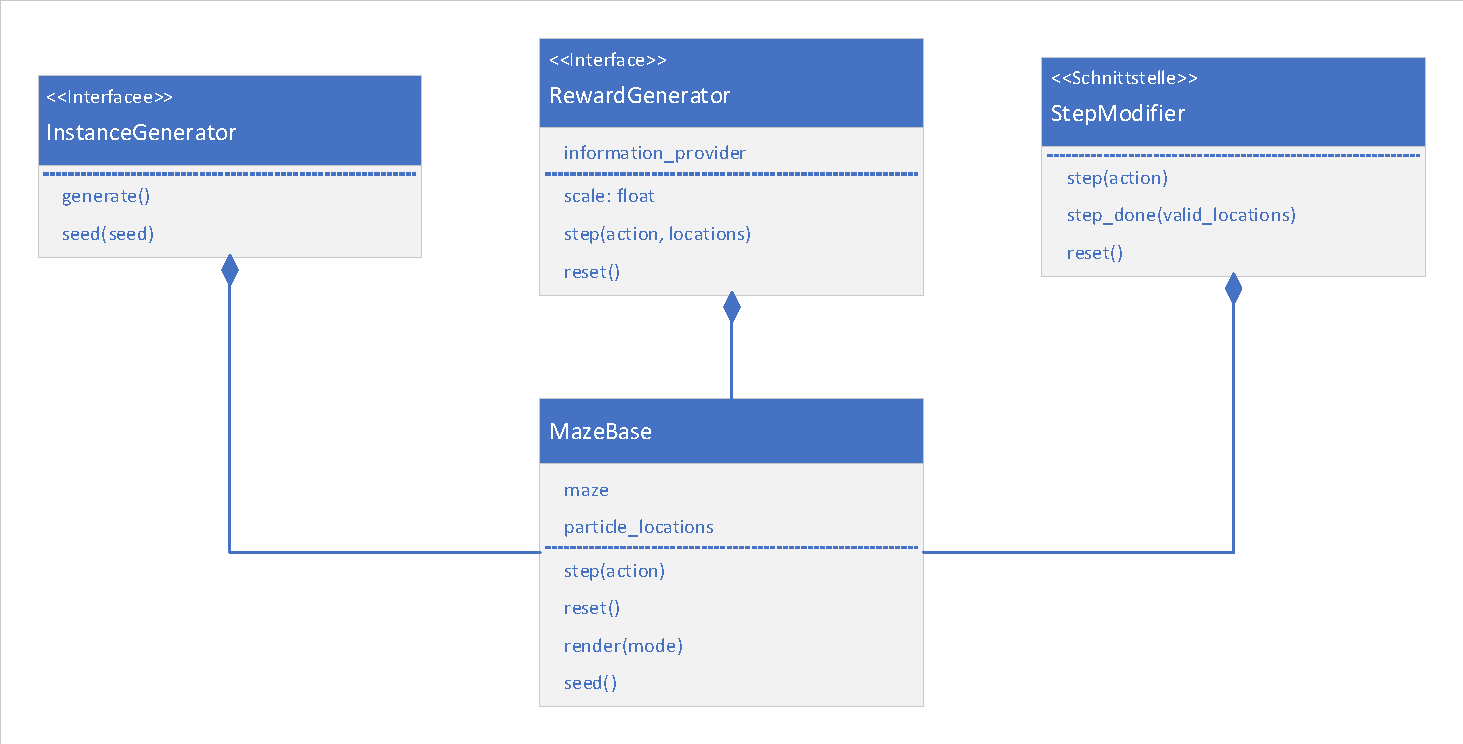
\includegraphics[clip, trim=10px 10px 10px 10px, width=0.9\columnwidth]{figures/implementation/maze_base_design.pdf}
    \end{center}
    
    %\vspace*{-6pt}
    \caption[Implementation Design for the Maze Environment]{Implementation Design for the Maze Environment.}
    \label{fig:MazeBaseDesign}
    %\vspace*{-12pt}
  \end{figure}

All components of the maze environment are generally designed with performance in mind. When implementing particle motions and reward generations, we minimized the use of python loop statements and instead solved most of the computations by utilizing NumPy \cite{oliphant2006guide} functions.

\subsection{Implementation Details} \label{sec:MazeImplementationDetails}
In this section we want to talk about technical details of our implementation. We will talk about the interface between the environment and the agent, how observations are generated and how we optimized the environment for speed. We also compare our implementation to the previous implementation of L. Huang \cite{huangMazeGithub}.

\paragraph{Agent Interaction.}
Like every environment which we want to use with Baselines Lab, the particle maze environment inherits from the OpenAI Gym base class \texttt{gym.Env} (see Section \ref{sec:BLExampleUsage}). The core method for the environment therefore is the \texttt{step} method. During training, all of the agent-environment interaction will happen by calling step with a selected action and receiving the observation and reward in return. The step method therefore must update the environment and create a new observation together with the reward for the selected action. Because step will be called thousands or even millions of times during each training session, all sub-methods called by step must be as lightweight as possible. We want to explain how we optimized the step method in a moment, but first we want to talk about the general concept of the maze environment.

The maze environment has to keep track of two things: The maze and the particles. We store both of these using 2-dimensional NumPy arrays. The maze is stored in two versions: One containing \textit{true} if the field is blocked and \textit{false} otherwise and an inverted version containing \textit{true}, if the field is not blocked and \textit{false} otherwise called freespace. This choice is not the most memory efficient, but will save some computation time when computing observations. We store the particle positions in a list-like structure, containing an entry for each particle with its (y, x) position. 

\begin{figure}[htp]
    \begin{center}
        \begin{tabular}{c}
            \parbox{0.9\columnwidth}{\inputpython{figures/implementation/code/loop_check.py}{0}{5}} \\
            \addlinespace[0.05cm]
            {\small (a) Native Python code.} \\
            \addlinespace[0.5cm]
            \parbox{0.9\columnwidth}{\inputpython{figures/implementation/code/no_loop_check.py}{1}{2}} \\
            \addlinespace[0.05cm]
            {\small (b) Python code with NumPy} \\
            
        \end{tabular}
    \end{center}
    \vspace{-0.25cm}
    \caption[Example for Python Loop Substitution with NumPy]{Example for substituting a Python loop with a NumPy statement. The array freespace is a 2d array containing false for blocked and true for non-blocked pixels. The locations array is a list of particle positions. NumPy arrays allow for advanced indexing, e.g. with a number of tuples. We also can index multiple dimensions of the array at the same time. Using these advantages, we can convert the Python loop from (a) into a single line of NumPy code in example (b).} \label{fig:MazeImplementation/Loops}
\end{figure}


\paragraph{Code Optimization. }
In order to optimize the code, our main concern is the execution speed of Python. Because Python is an interpreted language, the execution is slow when being compared to natively compiled languages like C. We therefore need to take advantage of libraries written in such a language to accelerate our code. The largest difference can be achieved, by eliminating loops from Python code. This can be easily demonstrated by a simple example: Let us say, we want to check which of our particles may have moved to a blocked pixel. We could do this, by iterating through the particles and check for each particle if its current position is not blocked using the freespace array  as demonstrated in Figure \ref{fig:MazeImplementation/Loops} (a). An alternative, which uses NumPy arrays can achieve the same result without the loop using just a single line statement as demonstrated in Figure \ref{fig:MazeImplementation/Loops} (b). 

\begin{figure}[htp]
    \begin{center}
        \begin{tabular}{c}
            \parbox{0.95\columnwidth}{\inputpython{figures/implementation/code/collision_detection_vanilla.py}{0}{9}} \\
            \addlinespace[0.05cm]
            {\small (a) Using native Python code only.} \\
            \addlinespace[0.5cm]
            \parbox{0.95\columnwidth}{\inputpython{figures/implementation/code/collision_detection_numpy.py}{0}{5}} \\
            \addlinespace[0.05cm]
            {\small (b) Using NumPy to eliminate loops.} \\
            \addlinespace[0.5cm]
            \parbox{0.95\columnwidth}{\inputpython{figures/implementation/code/collision_detection_numpy_2.py}{0}{7}} \\
            \addlinespace[0.05cm]
            {\small (c) Using single dimensional indexes instead of 2d-indexes.} \\
            
        \end{tabular}
    \end{center}
    \vspace{-0.25cm}
    \caption[Examples for Collision Detection using NumPy]{Examples for our collision detection system using different approaches. (a) uses a pure Python approach, while (b) and (c) use NumPy to accelerate computation. (c) uses a different indexing method than (b), by changing the multidimensional index from (b) to a single dimensional index by flattening the array.} \label{fig:MazeImplementation/Collision}
\end{figure}

Avoiding loops - especially when manipulating arrays - can save a lot of time, since the same operations may be executed hundreds or thousands of times for a single call. When it comes to array manipulation, NumPy (which is written in C) offers a lot of methods, which allow us to completely avoid Python loops even for complex operations. In Figure \ref{fig:MazeImplementation/Collision} (b), we show how we managed to perform the collision detection between particles and maze using solely NumPy statements. We also provide an alternative implementation using only native Python code in Figure \ref{fig:MazeImplementation/Collision} (a). Both implementations receive an action, the freespace array and the current location of the particles. They translate the action into the change of particle position using a global variable called \texttt{action\_map}. The native Python implementation then uses a loop to check for each particle if changing its position according to the action results in a new valid position and updates the location if this is true. This NumPy implementation first computes all new locations, ignoring collisions in Line 1. It then computes if these positions are valid in Line 2 and selects only valid positions in Line 3. 


We compare the speed of both implementations in Table \ref{tab:MazeImplementation/CollisionDetectionSpeed}. We can see, that avoiding Python loops significantly improves performance and also scales very well with increasing instance sizes and particle numbers. Note that the native Python implementation uses lists instead of NumPy arrays.


\begin{table}[htp]
    \begin{center}
        \begin{tabular}{crrrr}
            \toprule
            \multicolumn{1}{c}{Instance Size} & \multicolumn{1}{c}{Particle Count} & \multicolumn{1}{c}{Native} & \multicolumn{1}{c}{NumPy} & \multicolumn{1}{c}{NumPy Flattened} \\
            \midrule
            (100x100) & 64 & 9.27s & 1.34s & \textbf{1.22s} \\
            (100x100) & 256 & 16.32s & 1.62s & \textbf{1.55s} \\
            (100x100) & 1024 & 41.77s & 2.61s & \textbf{2.56s} \\
            \midrule
            (150x150) & 64 & 17.66s & 1.31s & \textbf{1.24s} \\
            (150x150) & 256 & 24.90s & 1.64s & \textbf{1.59s} \\
            (150x150) & 1024 & 52.43s & 2.66s & \textbf{2.59s} \\
            \midrule
            (200x200) & 64 & 28.13s & 1.26s & \textbf{1.22s} \\
            (200x200) & 256 & 35.05s & \textbf{1.57s} & 1.61s \\
            (200x200) & 1024 & 61.50s & 2.67s & \textbf{2.60s} \\
            \bottomrule
        \end{tabular}
    \end{center}
    \caption[Speed Comparison for Different Collision Detection Implementations]{Speed comparison for different implementations of the collision detection. Each run was executed with 100k randomly generated actions for the particle movement. We can see, that the pure Python implementation is significantly slower than a NumPy supported implementation. Both NumPy implementations also scale very well and are only affected by the number of particles due to the improved array structure (the Python implementation uses lists). The NumPy implementation with a flattened array is slightly faster in almost every test compared to the non-flattened implementation (see bold results).} \label{tab:MazeImplementation/CollisionDetectionSpeed}
\end{table}

Additionally using NumPy methods for all array manipulation tasks, we also tried to compare NumPy implementations with each other. Often there are multiple possibilities to solve the same problem using NumPy and not all of them have the same speed. Sticking to our collision detection example, we included an alternative implementation using also NumPy in Figure \ref{fig:MazeImplementation/Collision} (c). The only difference to the example in Figure \ref{fig:MazeImplementation/Collision} (b) is in Line 2. Instead of using the particle locations directly to index the two-dimensional array, we first flatten the array and then use a single dimensional index. For NumPy, this single dimensional index is faster, which can be seen, by comparing the results in Table \ref{tab:MazeImplementation/CollisionDetectionSpeed}.

\begin{table}[htp]
    \begin{center}
        \begin{tabular}{lrr}
            \toprule
            \multicolumn{1}{c}{Environment} & \multicolumn{1}{c}{Old Implementation} & \multicolumn{1}{c}{New Implementation} \\
            \midrule
            Corridor & 63.75s & \textbf{6.54s} \\
            Capillary & 68.41s & \textbf{7.66s} \\
            Brain & 160.22s & \textbf{12.31s} \\ 
            \bottomrule
        \end{tabular}
    \end{center}
    \caption[Maze Environment Implementation Speed Comparison]{Comparison between the environments implemented by L.Huang \cite{huangMazeGithub} and our implementation. The performance is measured in seconds for the execution of the step-method on different instances (see Section \ref{sec:TestProcedure} for a list of instances). The best value is marked in bold. Each environment performs 100k random actions with 256 particles and is automatically reset after performing 2000 steps. We can see, that our new implementation significantly reduces interaction time and also scales better with larger environments.} \label{tab:MazeImplementation/ImplementationComparison}
\end{table}

Previous implementations like the implementation of L. Huang \cite{huangMazeGithub} also used NumPy. We compared the difference in execution time between the different implementations on three test instances (see Section \ref{sec:TestProcedure} for a description of the instances) and listed the results in Table \ref{tab:MazeImplementation/ImplementationComparison}. We can see, that our new implementation significantly reduces agent-environment interaction time, being between 10 and 13 times faster.

\paragraph{Observations. }
We finally want to talk about the observations that are generated by the environment, which are similar, but not equal to previous implementations. The agent receives a single channel (greyscale) image where the maze is shown with blocked pixels being set to 255 and non-blocked pixels being set to zero. The positions of the particles are marked with a fixed value, independently of the number of particles gathered at a single pixel. Previous implementations used to mark more than a single pixel for each particle and instead marked a area of nine pixels around its center in the observation. 

In the case of random goal positions, we add two elements to the observation input: A circle around the goal position, indicating the goal range, and a square with side lengths of 3 pixels, centered at the goal position. Both the circle and the square also have their individual value, which is different from the value used to mark the positions of the particles. 

\subsection{Reward Shaping} \label{sec:MazeReward}
Rewards are a fundamental component of reinforcement learning. For RL algorithms the difficulty of a problem can largely depend on how much information the reward signal provides during training. Problems become especially complicated when dealing with very sparse rewards (e.g. just a single reward at the end of an episode). When designing a reward signal for a problem, it is therefore desirable to include as much information as possible into the reward signal to obtain faster and better learning results. Providing much information with the reward signal can include a risk though: The reward must be unbiased and should not limit the solution space the algorithm can come up with. If we reward specific strategies, the RL algorithm will just replicate that strategy and not learn anything new.

Keeping in mind that we want to create an unbiased reward signal, we can use the simple distance to the goal position as a measure for the reward signal. Since pixel perfect navigation is hard for RL algorithms, we want to allow slight inaccuracy and define a small area around the exact goal position in which we accept the solution. We then can measure the distance to the goal position for each particle and create two distinct reward signals from this measure:

\begin{itemize}
    \item \textit{Total cost reward} is generated based on the sum of distances $d_{total}$ of all particles to the goal position. A positive total cost reward therefore indicates overall improvement. This reward may also be generated by calculating the average cost $d_{avg}$ instead of the total cost.
    \item \textit{Max cost reward} is generated based on the particle with the greatest distance to the goal position $d_{max}$ only. This reward may differ significantly from the total cost reward, since it strongly punishes leaving behind single particles. 
\end{itemize}

As we mentioned in Section \ref{sec:TDDRL}, Huang et al. used both, the maximum and the total cost reward signal. Instead of giving a continuous reward signal, they defined 4-8 subgoals for both these values and only rewarded the agent if it was able to reduce the distance for the average or maximum particle below one of the subgoal thresholds. An example for this method is shown in Table \ref{tab:OriginalRewards}.

\begin{table} [ht]
    \begin{center}
        \begin{tabular}{|c|c|c|}
            \hline
            Max Cost & Reward & Completed \\
            \hline
            <10 & 8 & False \\
            <20 & 8 & False \\
            <40 & 4 & False \\
            <80 & 4 & True \\
            <120 & 2 & True \\
            $\vdots$ & $\vdots$ & $\vdots$ \\
            \hline
        \end{tabular}
    \end{center}
    \caption[Original Reward Example]{Example for the original reward system. By reaching a certain goal for a reward category (e.g. max cost) the agent is rewarded with a certain reward. Each reward can only be obtained a single time \cite{huang2019}.} \label{tab:OriginalRewards}
\end{table}


The sparseness of this reward signal may significantly increase the complexity of the problem. Also this reward is not flexible, since the reward subgoals were handcrafted for each individual instance. In order to investigate the impact of different rewards, we test a number of combinations of our reward components and measure their impact on the performance in Section TODO. In the following we want to explain what the goal behind each reward component is and how we calculate them. Figure \ref{fig:RewardDesign} provides an overview of the different components of our flexible reward system.

\begin{figure}[ht]
    
    \begin{center}
        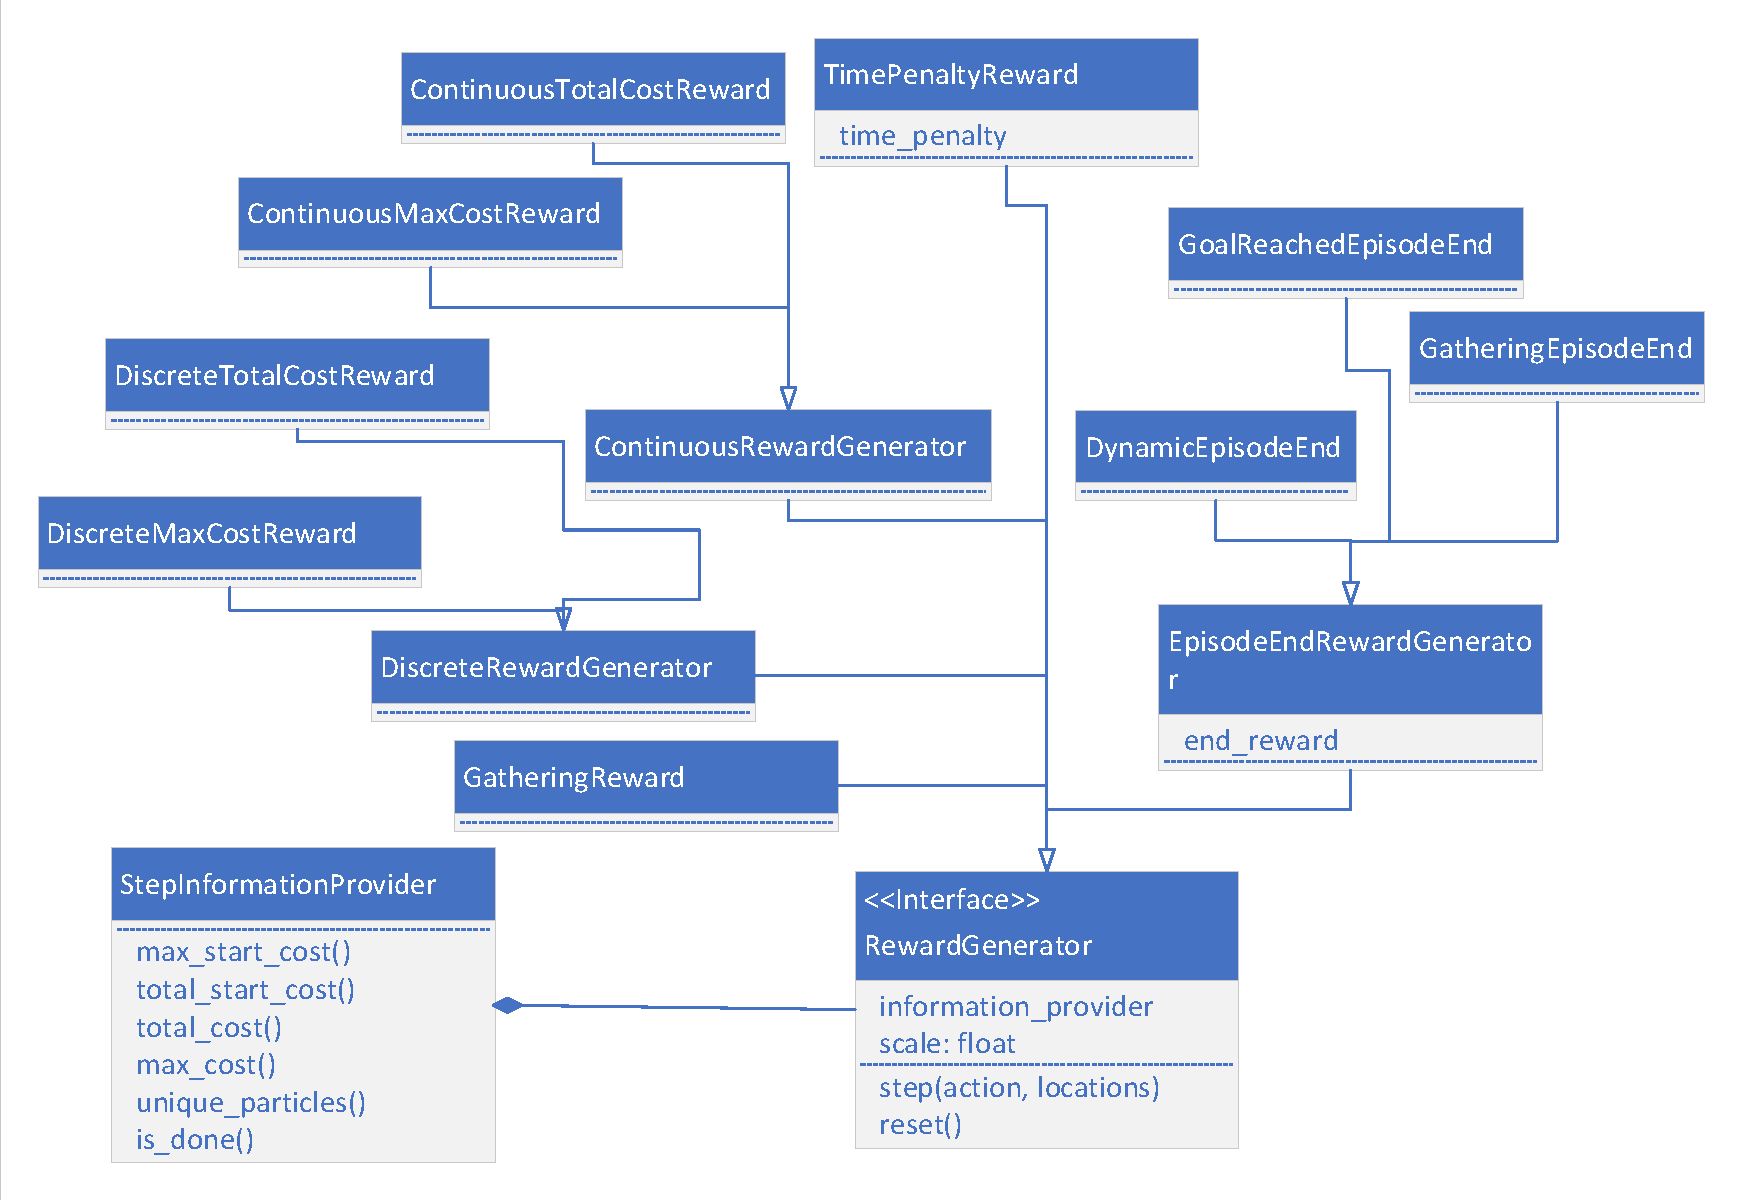
\includegraphics[clip, trim=10px 10px 10px 10px, width=0.95\columnwidth]{figures/implementation/reward_design.pdf}
    \end{center}
    
    %\vspace*{-6pt}
    \caption[Implementation Design for the Reward Generators]{Implementation design for the reward generators. To improve efficiency, all reward components share an object called of the type \textit{InformationStepProvider} which ensures that the same calculations are not repeated multiple times.}
    \label{fig:RewardDesign}
    %\vspace*{-12pt}
\end{figure}

\paragraph{Discrete Reward.}
We implemented a reward which works similar to the original reward, but with a dynamic number of subgoals. We also drastically increased the number of subgoals, to make the reward less sparse. Instead of rewarding the agent at 4-8 subgoals (which in the original implementation were all given to the agent if its solution was already close to the goal position) we dynamically compute a number of subgoals depending on the size of the maze and distribute these subgoals evenly. This way the agent already receives reward at early stages of the training process. We estimate the number of subgoals by halving the maximum distance any particle can be away from the goal position. Subgoals which are easier to reach (the first subgoals) generate a smaller reward than later ones.

\paragraph{Continuous Reward.}
To reduce sparseness to a minimum, we also implemented continuous reward. The continuous reward does not define any subgoals and instead directly rewards the agent by the change in distances for both, the maximum and the total cost metric. In this case it is important to either use the average cost metric or scale both the total distance metric and the maximum cost metric to $[0, 1]$, otherwise the weight of the total distance metric is much larger than the weight of the maximum cost metric. There is a second aspect to using scaled total distance reward though and that is reward consistency: Larger instances would automatically generate more reward if the reward is directly dependent on the distance between particles and the goal position. If we want to explore agents which can solve randomly generated instances, we need a reward which always has the same total sum over an episode. We call the the continuous reward normalized, if both the total cost and the maximum cost metric are scaled to $[0, 1]$ (so the reward is always bounded to $[0, 2]$). 

One problem when creating the continuous reward signal only based on the change in the particle distance is, that the same observation does not always create the same amount of reward. Remember when we talked about the idea of a baseline in Section \ref{ssec:ImprovingPG}? The problem was, that in most situations a high or a low reward does not tell us if the agents performance is good, because the starting situation for the agent might be better or worse than average just by chance. Therefore modern RL algorithms already account for these fluctuations by estimating how good the current state is. For optimal performance, we therefore must design a reward signal, which is consistent through multiple executions for the same environment state - rewarding the agent even if it has just been lucky.

To achieve this, we need an estimate for the starting cost for both the maximum and total (or average) cost metric, which is independent of the actual particle positions. For the total cost metric, we can use the total distance of each possible particle position to the goal position and for the maximum cost metric we use the maximum distance a single particle can be away from the goal position. For each step of training, the continuous reward is then calculated by subtracting the current value of each metric from the corresponding value after the last step. 

Generating totally continuous reward may discourage the agent to gather particles which got stuck at some point, if it has to move other particles away from the goal position, because it may receive large amounts of negative reward in the process. We therefore propose an extension to the continuous reward signal which cuts off negative rewards and returns zero reward for all steps which would otherwise result in a negative reward.

\paragraph{Time Penalty.}
While the basic reward does encourage the agent to bring all particles to the goal position, there is no pressure on the agent to use a minimum amount of time. It will receive the same amount of reward independent of the total time. To add a time constraint, we can add a time penalty to the reward signal, which is given out at each step. The original implementation used a static time penalty of $-0.1$ reward per step. With our dynamic reward system this static time penalty does not work optimally for two reasons: First, the ratio between time penalty and the rest of the reward signal may not be the same for all environments, since larger environments now provide more reward due to particles being further away (except for normalized continuous reward). Second, larger environments may need more time to solve and - like before - we are interested in a constant total value for the time penalty. The problem here is that we do not know beforehand what the optimal episode length will be. We therefore propose to estimate the optimal episode length by

\[ep\_len \approx 0.75 * d_{max} * \log (d_{avg} * k)\]

Here $d_{max}$ is an estimate for the maximum distance between any two points of the maze, by using the maximum distance between a random extreme position and any other point in the maze. $d_{avg}$ is the average distance between any point and the goal position and $k$ is the number of convex corners. We experimentally found, that the constant factor $0.75$ works best to estimate the number of steps needed to solve the environment across our test instances.

The time penalty is given by $ep\_len^{-1}$. For discrete or unnormalized continuous rewards, we scale this time penalty to match the sum of all rewards. 

\paragraph{Gathering Reward.}
Bringing the particles to the goal position requires to gather the particles in a small area or even in a single pixel. We therefore create an additional reward signal which is generated by calculating the number of unique particle positions in the current step. This reward signal can also be normalized to $[0, 1]$ by dividing it by the initial number of particles. Note that gathering reward might also be more complex by calculating the total pairwise particle distance, but this calculation is extremely costly and we therefore did not use this option.

\paragraph{Dynamic Episode Length.}
When training an agent on the maze environment, we usually set an upper time limit to the maximum episode length. When training the agent it usually receives more and more reward over time until it is able to solve the environment and the episode length decreases. With the addition of curiosity reward, this produces a problem: Longer episodes are usually more interesting. This was observed in the RND paper \cite{burda2018exploration} and during our verification experiment (see Section \ref{sec:blRND}). This means, that adding a curiosity reward to the agent may encourage the agent to not find a solution which brings all particles on the shortest path to the goal position. This problem can be solved to some extend, by scaling down the curiosity reward, but the problem itself is still present. 

There is also a second aspect when talking about the time limit. A high time limit may lead to training situations, where the agent gets stuck at some point and then is not able how to figure out how it should get out of the current situation. By resetting the environment the agent may find a strategy which completely avoids the situation from before. A high time limit therefore might impact the training performance negatively, if the agent gets stuck in a state and then has to wait until the episode is over and it can try again. On the other hand a very short time limit can also negatively impact training. The limit may be shorter than the shortest possible solution and a short time limit also decreases the possibility for exploration. We therefore need to estimate an ideal episode length. 

When we talked about the time penalty, we already proposed a way to estimate the optimal episode length. Using this value as an upper limit would make sense, but we could also go one step further: Since we are dealing with non-sparse rewards, we could monitor the reward during an episode to detect situations in which the agent got stuck. We then dynamically cancel episodes which are not promising. To achieve this, we divide the estimated episode length by the number of expected positive rewards. In the case of discrete rewards, this is the number of subgoals. We then increase the time limit each time the agent is able to gain a positive reward. We also include a small bias, which gives the agent a little bit more time early on and a little bit less time the longer the episode has already been.

Using a dynamic episode length in this form may cause problems in combination with a time penalty. Since longer episodes result in more time penalty (meaning less total reward), the agent might try to end episodes as fast as possible. In the case of dynamic episode lengths a short episode means not receiving any "normal" reward at all. We therefore add two constraints which should resolve this problem: First, if the agent is not able to reach the goal, it will receive a negative reward equal to the time penalty it would receive if the episode had not been canceled early. Additionally, if the agent is able to finish the episode earlier than the estimated episode length, it receives a positive reward which is proportional to the number of steps its solution was faster than expected.

\subsection{Extended Models} \label{sec:ExtendedMaze}
Previous work only looked at the particle navigation problem from a very theoretical point of view. Each particle could be perfectly observed meaning we always had information about its pixel perfect position. We also were able to perfectly apply the same uniform transformation to each particle and this transformation was a direct change of the position instead of a "real" movement. To investigate the performance of RL models under more real-life conditions, we therefore implemented two extensions which we evaluated one-by-one and combined in Section TODO.

\paragraph{Introducing Error.}
When it comes to real world applications, we always will have to deal with multiple sources of error. Sensors will always provide a certain amount of noise and actions might not be executed perfectly. To simulate various error sources we therefore introduce fuzzy observations and fuzzy actions.  

In combination with noise, detecting the exact location of microscopic particles will always be inaccurate as particles may not be recognized correctly. We therefore generate fuzzy observations by using three possible sources of error:

\begin{itemize}
    \item \textit{Noise.} To simulate standard detection error, we add gaussian noise to the observation.
    \item \textit{False Negative Detection.} At each step, each particle has a small chance to be not be included in the observation at all.
    \item \textit{False Positive Detection.} At each step, particles with random positions may be added to the observation.
\end{itemize}

While particles in the theoretical model are directed using a uniform force, in reality particle movement will never be completely uniform. Slight changes in the magnetic field, collisions with other particles or fluctuations in the blood flow, may interfere with the navigation at any time. Also the generation of the magnetic fields may work with a slight delay and that delay might change over time. We therefore generate fuzzy actions using three sources of error.

\begin{itemize}
    \item \textit{Sticky Actions.} Each action has the probability to be executed again for the next step.
    \item \textit{Noisy Actions.} Each action may only affect a certain percentage of the particles.
    \item \textit{Random Actions.} Each particle may move randomly at each step.
\end{itemize}

We test all these sources of error and their influence on the performance in Section TODO.

\paragraph{Physical Particles.}
While error in actions and observations adds a lot to the realism of the simulation, we are still working with particles which directly change from one position to another. Instead we want to have particles which behave more like real particles. Instead of directly changing the particle position, we want to accelerate particles. Particles themselves then have an internal speed vector which also influences their position for the following steps of the simulation. To simulate friction we divide this speed vector by a constant value of $1.1$ for each step and set the speed to zero if a particles' speed drops below a threshold. The particle position is rounded to match an integer position for the observation, but kept at floating point precision for internal calculations.

One problem when simulating physical particles is that the computations for the environment get more complicated and training needs more time. This is especially problematic when calculating collisions with the maze. For the non-physical particles, each particle could at most move a single pixel in any direction. If the particle was blocked by the maze in that direction it would remain at its current position. However with physical particles, particles may actually move more than one pixel per step. In case of a collision, we would need to calculate the exact point of contact between the particle and the maze. Instead we approximate the collision by halving the speed if the particle would cause a collision at full speed. The particle then does not move for the current step, but will keep half of its velocity for the next step, getting closer and closer to the wall. Note that this procedure might allow particles to move through walls if their velocity is large enough to cross the wall in a single step. However the size of our test instances does not allow the agent to accelerate particles to this point.

We investigate the performance of RL algorithms when dealing with physical particles in Section TODO.

\subsection{Random Instance Generation} \label{sec:RandomInstanceGeneration}
To train agents to solve randomized mazes, we need a generator which produces blood vessel like structures. To generate these structures we used an algorithm called \textit{rapidly-exploring random tree} (RRT) \cite{lavalle1998rapidly}. The algorithm was originally designed to efficiently search high-dimensional spaces by randomly generating a space-filling tree. The tree is generated by randomly proposing new points in the search space and connecting these new points to the closest point of the search tree. If the random point is to far away from the closest point of the search tree, a new node is inserted at a predefined maximum length in the direction of the random point. Using the RRT algorithm, we create blood-vessel like instances in four steps:

\begin{enumerate}
    \item Generate a new RRT. A low bound on the maximum length for each new segment ensures a river-like structure of the tree. Figure \ref{fig:RRRTrees} (a) shows an example RRT tree with 250 nodes.
    \item We calculate the \textit{flow} to the starting node of the tree. Each leaf node generates a flow of one and propagates that flow back to the root node of the tree (see Figure \ref{fig:RRRTrees} (b)).
    \item Create random loops in the tree, by generating a set amount of random points and connecting them to the two closest nodes of the tree. (see Figure \ref{fig:RRRTrees} (c))
    \item Draw the tree, using the square root of the flow value as width for each segment.
\end{enumerate}

\begin{figure}[ht]
    \begin{center}
    %\resizebox{0.95\columnwidth}{!}{%
    \begin{tabular}{cc}
    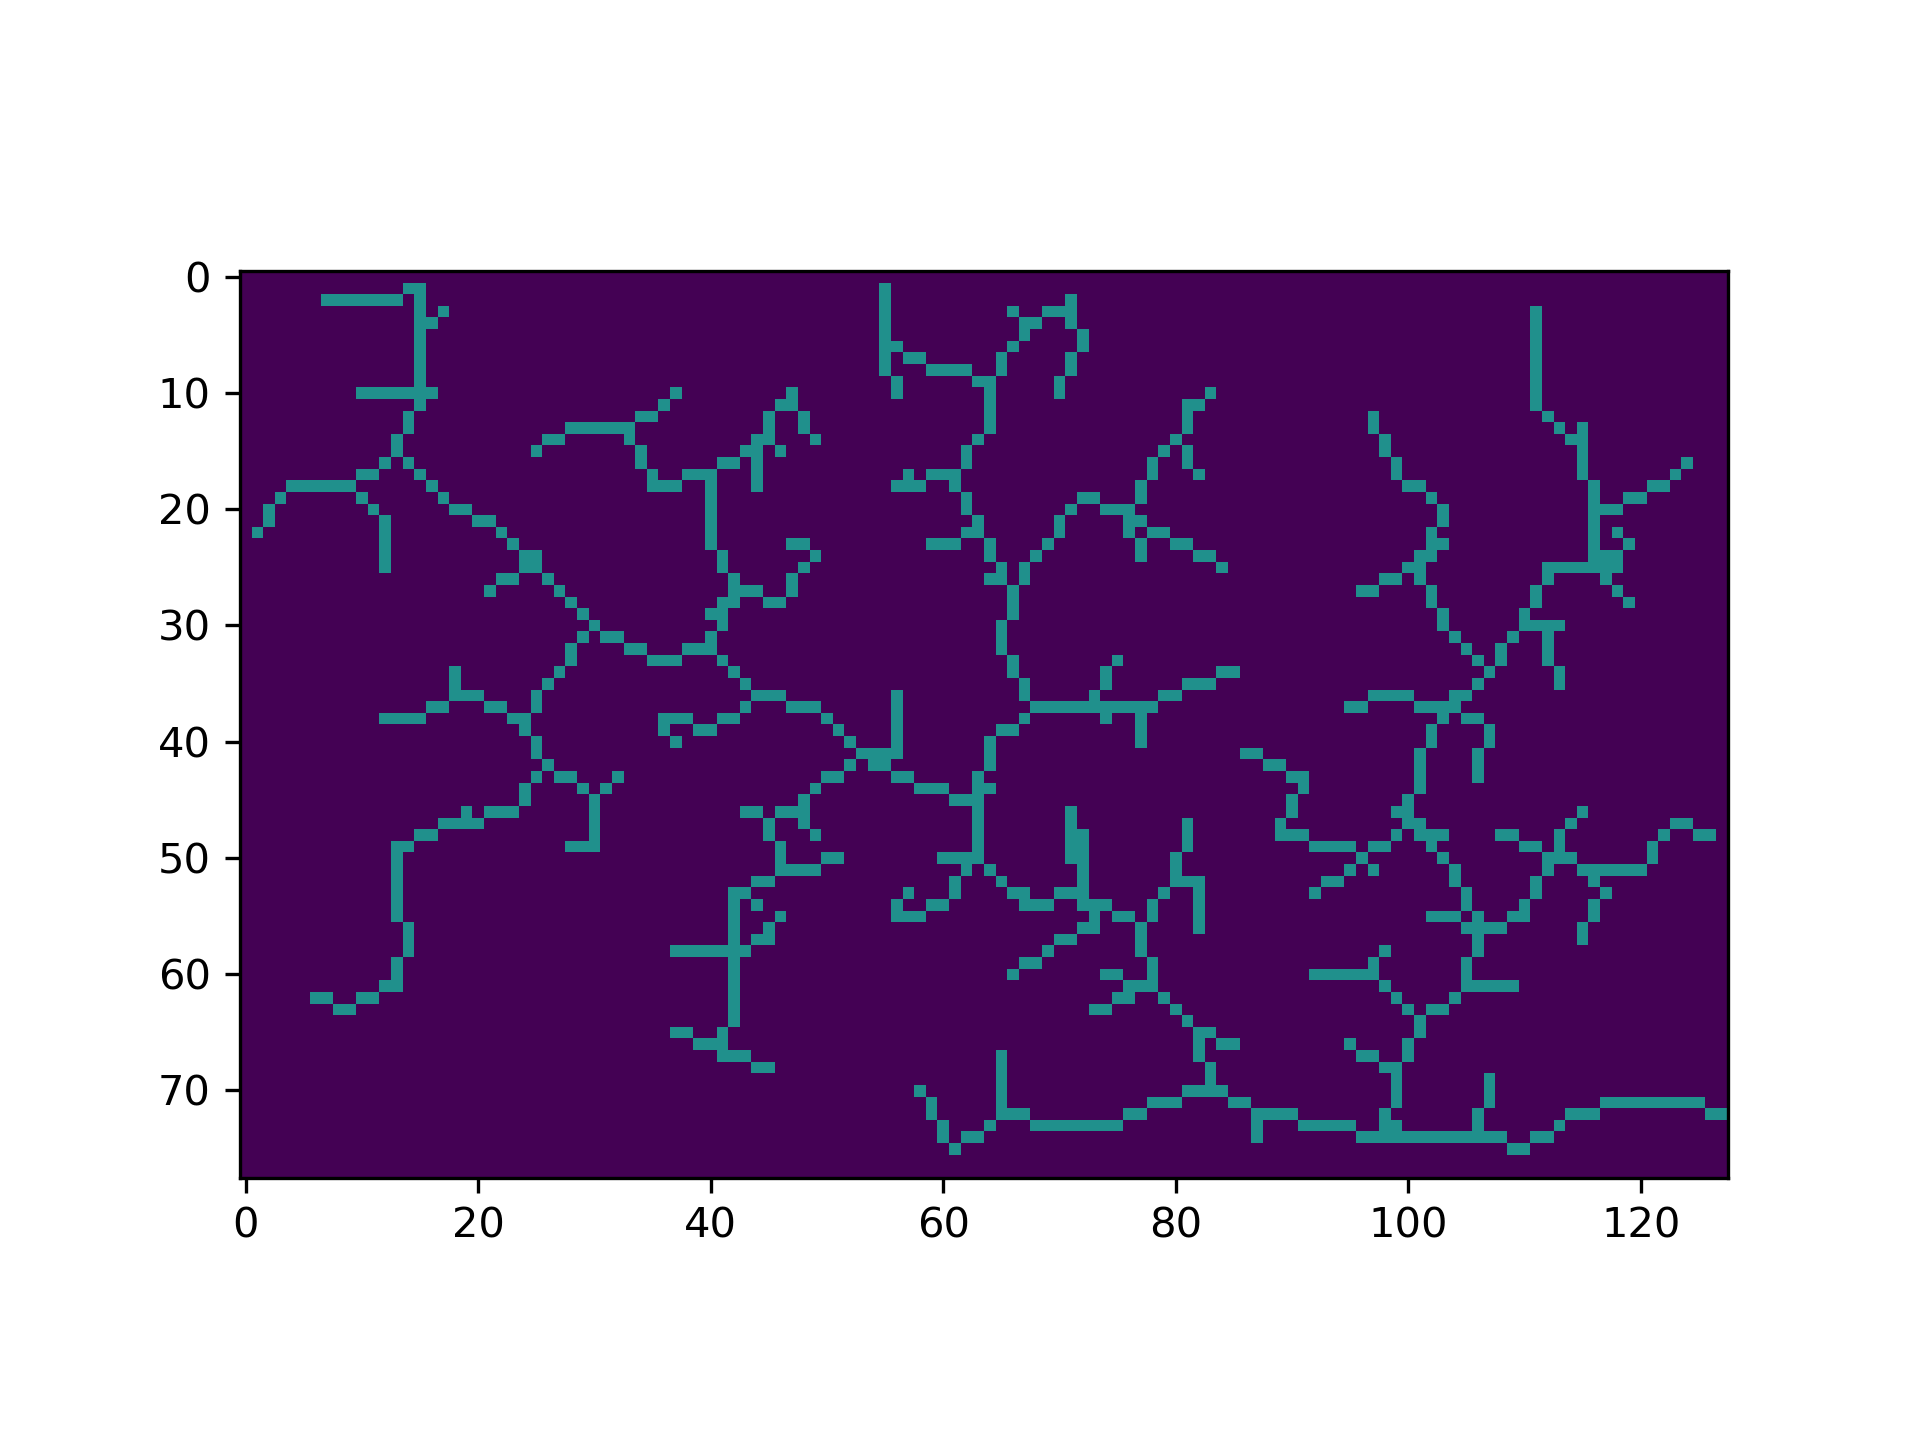
\includegraphics[clip, trim=58 62 45 60, height=3.5cm]{figures/implementation/rrt_base.png} &
    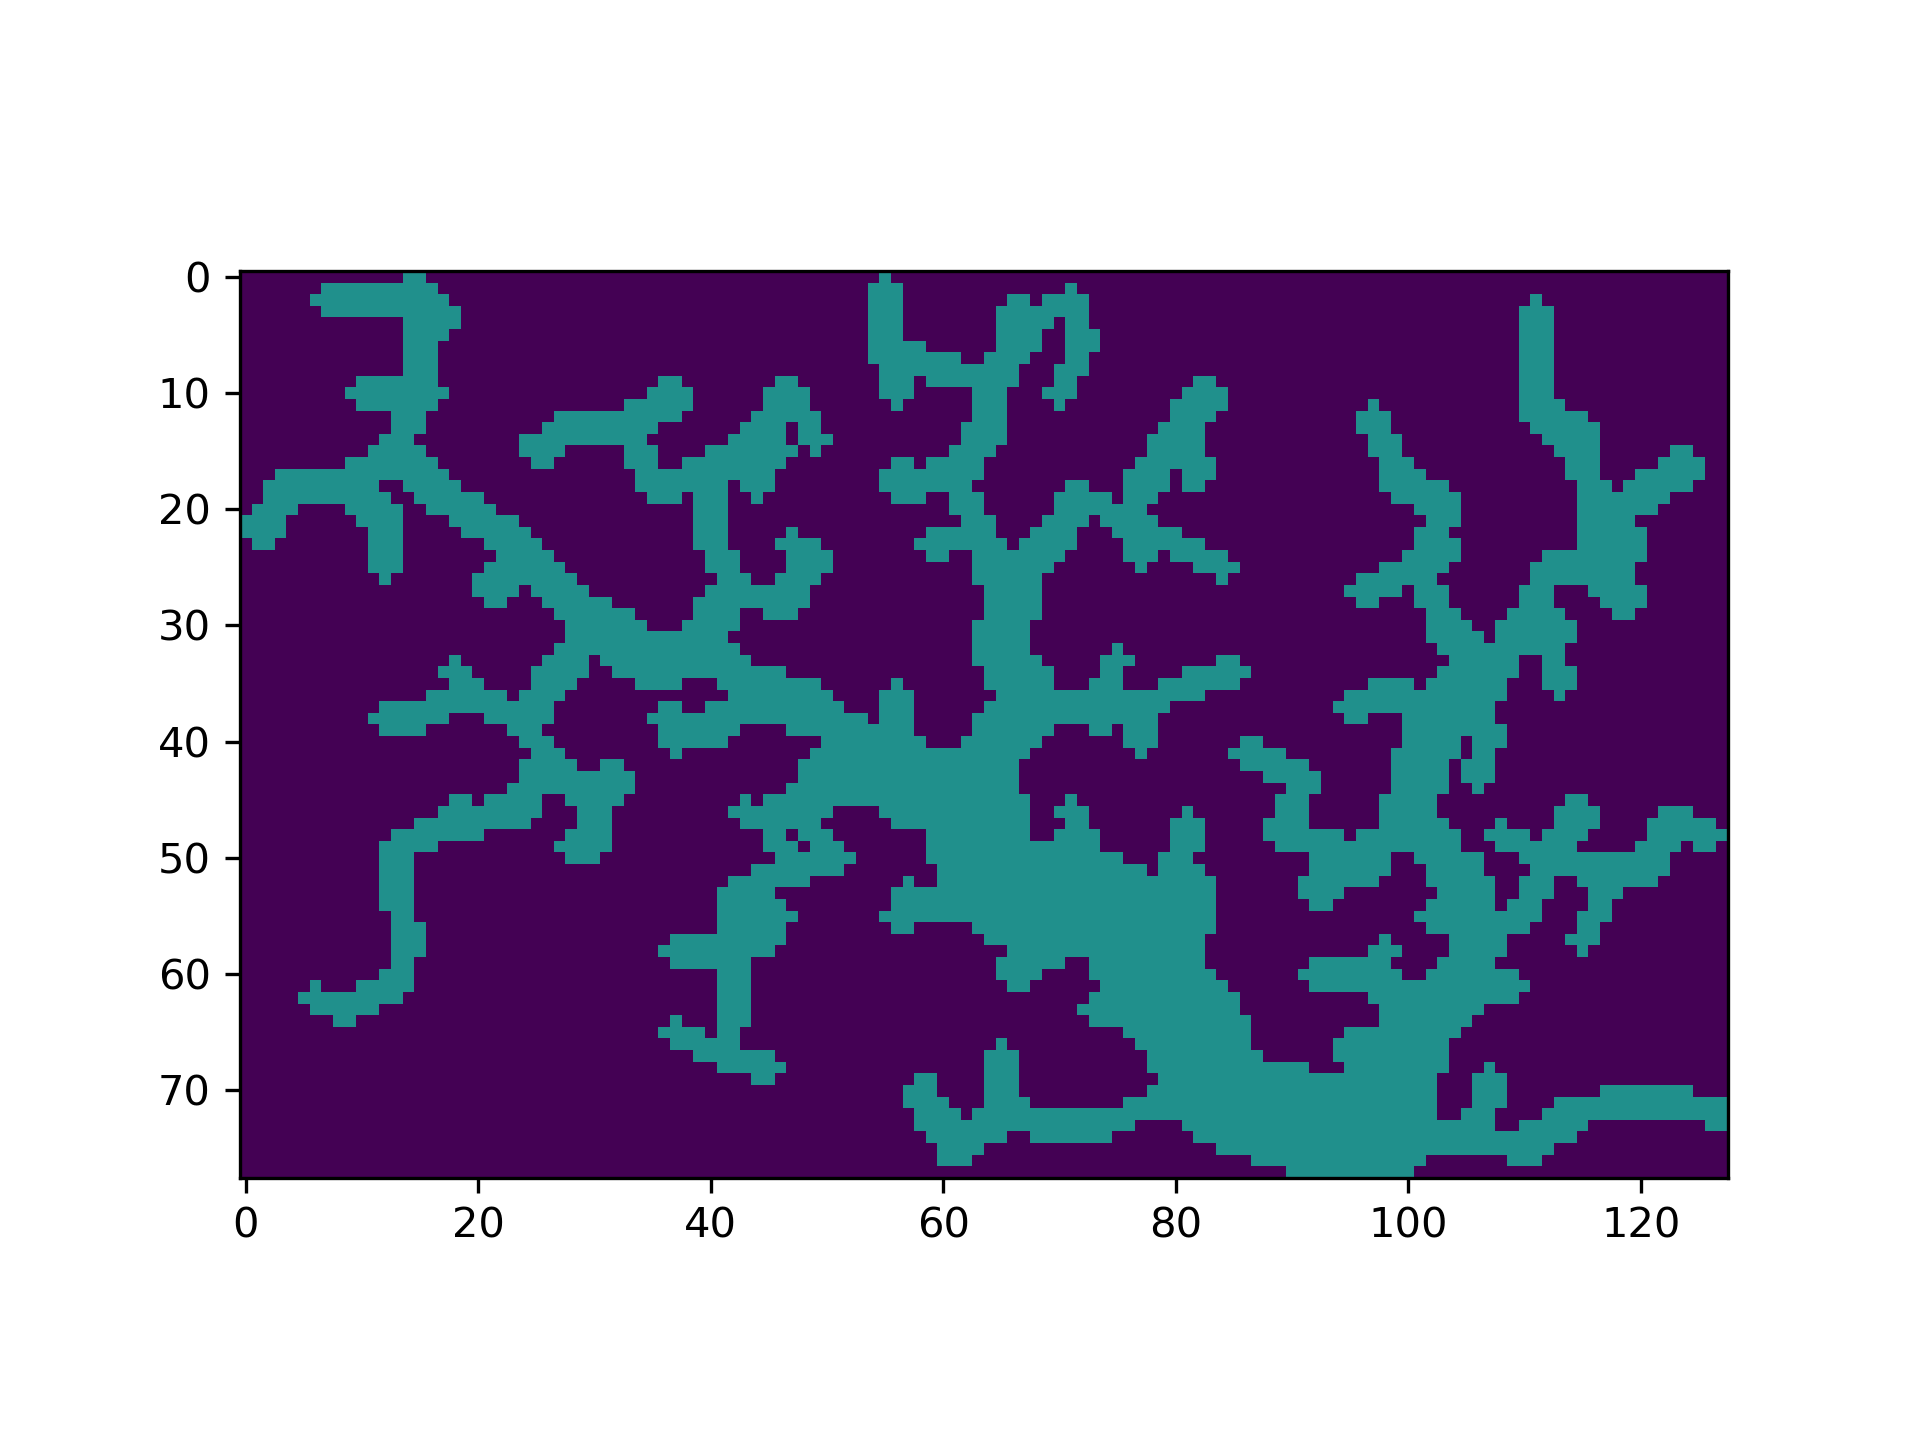
\includegraphics[clip, trim=58 62 45 60, height=3.5cm]{figures/implementation/rrt_base_flow.png} \\
    {\footnotesize (a) A simple RRT tree.} &
    {\footnotesize (b) Flow-based branch scaling.} \\
    \multicolumn{2}{c}{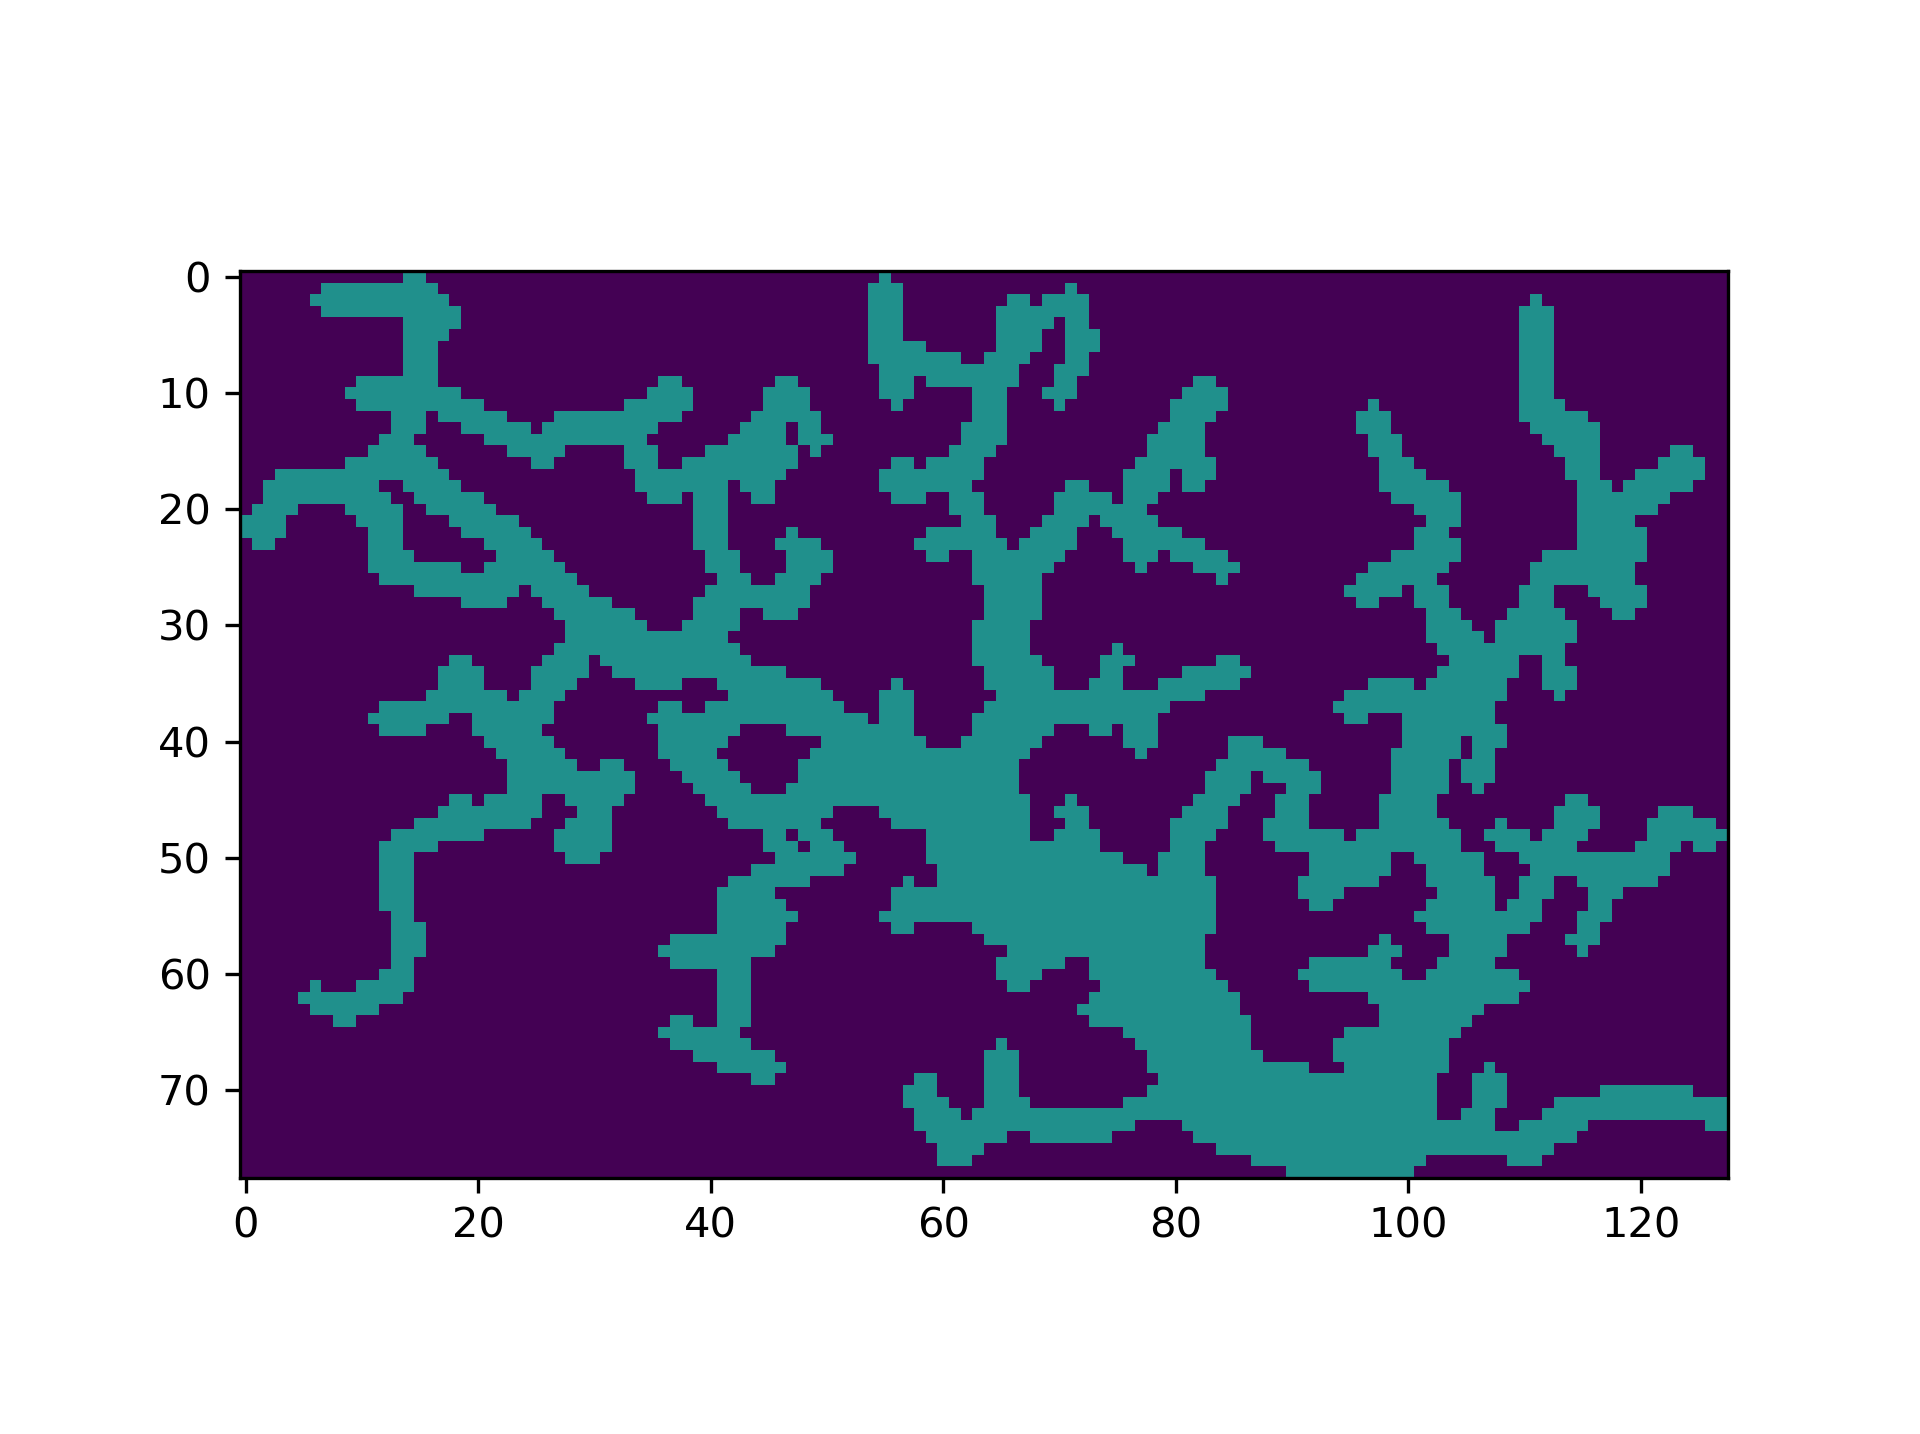
\includegraphics[clip, trim=58 62 45 60, height=3.5cm]{figures/implementation/rrt_base_loops.png}} \\
    \multicolumn{2}{c}{{\footnotesize (c) Adding random non-intersecting loops.}}
    \end{tabular}
    %}%
    \end{center}
    %\vspace*{-12pt}
    \caption[Random Instance Generation]{Creating vessel-like random instances with the RRT algorithm.}
    \label{fig:RRRTrees}
    %\vspace*{-12pt}
  \end{figure}

When training with randomly created instances a goal position is randomly chosen from the set of empty pixels. Additionally we buffer the randomly created instances and choose an already created instance with a probability of 95\% and only generate a new instance with a probability of 5\%. This avoids expensive recomputation at every environment reset.

\subsection{Integration of Algorithmic Approaches} \label{sec:AlgorithmIntegration}
To allow easy evaluation, we integrated an adapter which allows algorithmic strategies, which precompute all particle movements, to interact with our step-based environment and replay their decisions accordingly. By adapting code from \cite{becker2020} we have access to the SSP, DSP and MTE algorithms as shown in Section \ref{chp:TDD}. Evaluation results comparing the RL approach against the algorithmic approaches can be found in Section TODO.

